% ============================================================
% ［架空の記入例・提出不可］研究設定，データ，数値および結果はすべて架空である．
% 引用文献だけは実在する．構成，LaTeX記法および根拠密度の見本であり，
% 文章量の目標ではない．節見出し，本文，図表，数式および\cite{key}を含むが，
% \printbibliographyと\nociteは記載しない．
% main.texは埋込みアブスト用の一覧をアブスト内へ，本文用の一覧を巻末へ出力し，
% abstract.texは独立アブスト用の一覧を末尾へ出力する．
% ============================================================
\begin{center}
  \UsamiFictionalExampleNotice
\end{center}

\AbstractSection{1．はじめに}
2次元人物姿勢推定は，行動認識や作業支援へ人体構造を与える基盤技術である．低照度では局所コントラストが低下し，関節信頼度が高いまま肢長比の崩れた骨格を出力することがある．本研究では既存推定器を固定し，関節信頼度と骨格構造の一貫性から誤推定骨格を除外して，採用骨格の精度と採用率の関係を調べる．

対象は単一人物を含む切出し画像とし，提案処理は関節座標を補正せず，骨格を後段へ渡すか否かだけを判定する．したがって目的は全フレームの位置精度向上ではなく，許容する採用率の下で誤推定の流入を抑えることである．なお，以下の研究設定，データ，実験条件，数値および結果はすべて架空である．

\AbstractSection{2．関連研究}
HRNetは高解像度表現と複数解像度の反復融合により，高精度な関節位置推定を実現した\cite{sun2019hrnet}．ViTPoseはVision Transformerと軽量な復号器による単純な構成でも高い性能を示した\cite{xu2022vitpose}．本研究はこれらと異なり，推定器に依存しない出力判定を追加して，撮影環境の劣化時に後段へ渡す骨格を選別する．

\AbstractSection{3．提案・実施内容}
提案処理の流れを図\ref{fig:pipeline}に示す．固定した姿勢推定器から$J=17$個の関節座標$\hat{\bm{p}}_j$と信頼度$c_j$を取得し，人物単位の骨格品質スコア$q$を算出する．

\begin{center}
  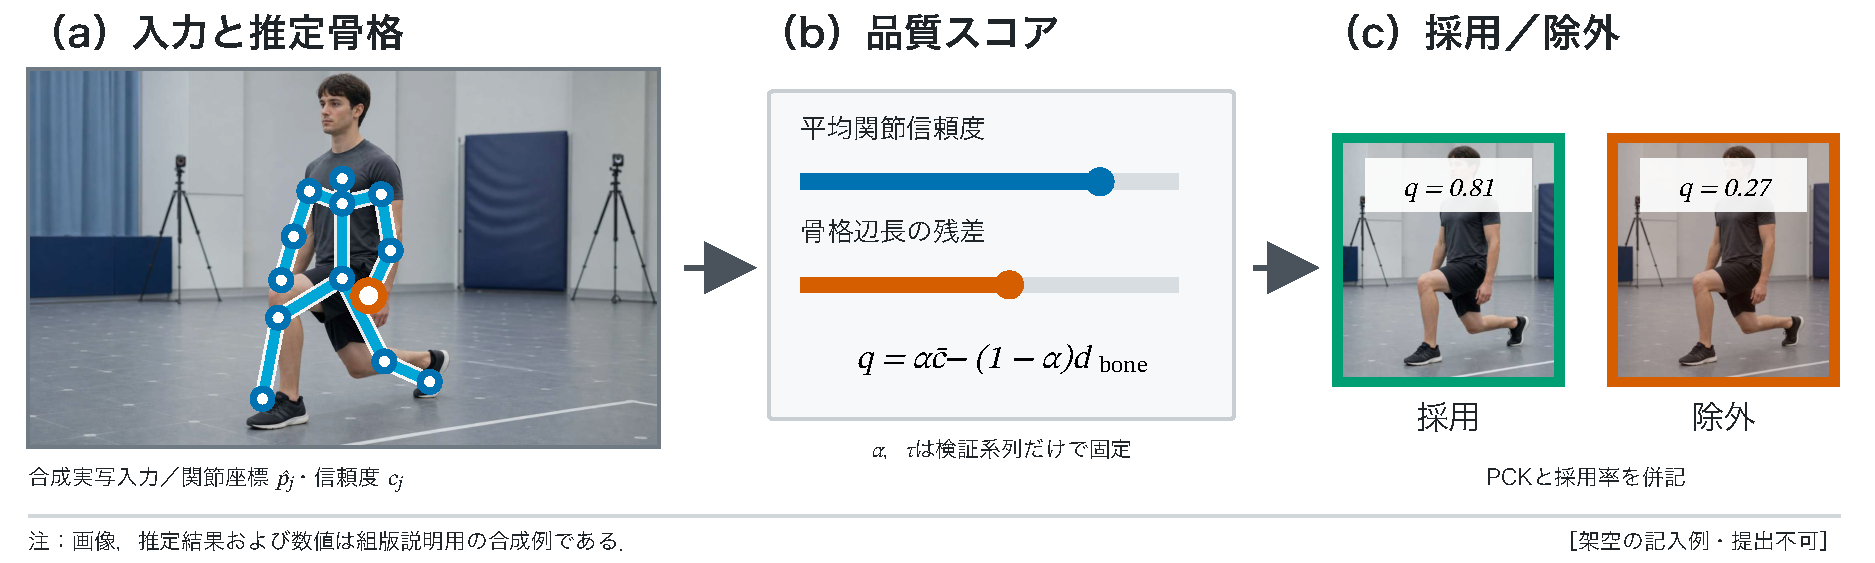
\includegraphics[width=\columnwidth]{examples/figures/pose-quality-abstract.pdf}
\captionof{figure}{誤推定骨格を除外する処理の流れ}
\label{fig:pipeline}
\end{center}

平均関節信頼度を$\bar{c}$，胴体長で正規化した骨格辺$e$の長さを$\tilde{\ell}_e$，学習系列におけるその中央値を$\mu_e$とする．$\mathcal{E}$はCOCO骨格の16辺とし，胴体長には左右肩中点と左右腰中点の距離を用いる．信頼度0.1未満の関節は欠損として$c_j=0$とし，胴体長が画像高の5\%未満なら正規化不能として除外する．骨格辺集合$\mathcal{E}$に対し，
\begin{equation}
  \begin{aligned}
    d_{\mathrm{bone}}
      &=\frac{1}{|\mathcal{E}|}\sum_{e\in\mathcal{E}}
        |\tilde{\ell}_e-\mu_e|,\\
    q&=\alpha\bar{c}-(1-\alpha)d_{\mathrm{bone}}
  \end{aligned}
  \label{eq:quality-score}
\end{equation}
と定義する．式\eqref{eq:quality-score}の$q<\tau$を除外し，$\alpha$と$\tau$は検証系列だけで決める．

$\mu_e$は学習系列だけから算出し，検証系列では$\alpha$と$\tau$の組を0.05刻みで探索する．評価前に推定器，$\mu_e$，$\alpha$，$\tau$を固定し，評価結果を見た再調整は行わない．図\ref{fig:pipeline}の判定はフレーム単位であり，前後フレームの推定結果は用いない．

\AbstractSection{4．実験・評価}
20--40 lxの室内で12名から各1系列200フレーム，計2,400フレームを収録し，各フレームの1名に17関節を付与した．人物単位で学習，検証，評価へ4系列ずつ分け，同一人物と隣接フレームの混入を防いだ．照度20，30，40 lxと直立，歩行，着座が各集合へ含まれるよう割り当てた．COCO事前学習済みHRNet-W32を$256\times192$画素入力で固定し，除外なし，平均信頼度，提案スコアを比較した．検証系列で採用率80\%以上のPCK@0.2を最大化し，$\alpha=0.65$，$\tau=0.42$を得た．PCK@0.2は胴体長で正規化し，採用骨格だけで算出する一方，採用率を必ず併記した．系列ごとに指標を求め，4系列を等重みで平均した結果を表\ref{tab:results}に示す．

\begin{center}
\small
\captionof{table}{低照度評価系列における誤推定骨格の除外結果（架空値）}
\label{tab:results}
\begin{tabular}{lcc}
\toprule
除外方法 & PCK@0.2［\%］ & 採用率［\%］ \\
\midrule
なし & 73.1 & 100.0 \\
平均信頼度 & 78.2 & 86.4 \\
提案スコア & \textbf{82.1} & 81.7 \\
\bottomrule
\end{tabular}
\end{center}

提案スコアは評価800フレーム中654フレームを採用した．系列別PCK@0.2は79.8--84.3\%，採用率は77.5--85.0\%であり，平均値が単一系列だけで生じたものではなかった．除外146フレームの目視分類では，遮蔽または動きぼけを伴う末端関節の誤推定が91，正しいが学習時の辺長分布から外れた姿勢が24，人物切出しのずれ等が31であった．

\AbstractSection{5．考察}
表\ref{tab:results}より，提案スコアは除外なしに対してPCK@0.2を8.9ポイント高めたが，採用率は18.3ポイント低下した．平均信頼度による除外と比べてもPCK@0.2は3.9ポイント高く，骨格辺長が高信頼度の誤推定を補足した可能性がある．一方，24フレームの有効姿勢を除外しており，学習分布から外れる屈曲姿勢を誤りとみなす偽除外が残る．また，関節間比率を保ったまま骨格全体が平行移動する誤推定，胴体の遮蔽，人物切出しの失敗は式\eqref{eq:quality-score}だけでは検出しにくい．本手法は位置を修正せず，難しいフレームを捨てて精度と採用率を交換するため，欠損を許容できない用途にはそのまま適用できない．単一室内・固定照度・単一推定器での評価であり，カメラ，人物属性，屋外光，時系列判定，後段タスクへの一般化は未検証である．

\AbstractSection{6．おわりに}
関節信頼度と正規化骨格辺長を統合し，低照度映像の誤推定骨格を除外した．信頼できる骨格だけを後段へ渡す構成には有用性があるが，実運用には複数カメラでの再評価と欠損骨格を扱う設計が必要である．
